%#!platex
\documentclass[platex,dvipdfmx]{rbproceedings}
% English option
%\documentclass[platex,dvipdfmx,english]{rbproceedings}
%#!uplatex
%\documentclass[uplatex,dvipdfmx]{rbproceedings}
%#!lualatex
%\documentclass[lualatex]{rbproceedings}

% パッケージ
\usepackage{graphicx,xcolor}  % グラフィックス関連
\usepackage{url}
\usepackage{hyperref}
\hypersetup{
    colorlinks=true,
    citecolor=blue,
    linkcolor=blue,
    urlcolor=blue,
    pdfborder={0 0 0},
}
%\usepackage{jlreq-deluxe}  % 多書体化(otf パッケージは使用しない)、Ubuntu 22.04 以降
\usepackage[verb]{bxghost}  % \verb 前後に適切な和欧文間スペース
\usepackage{pxrubrica}  % ルビ

% 参考文献のフォントサイズを指定
%\renewcommand{\bibfont}{\normalsize}  % 標準サイズ
%\renewcommand{\bibfont}{\footnotesize}  % より小さく

% \emph をゴシックかつ太字に(比較的新しい LaTeX が必要)
\DeclareEmphSequence{\gtfamily\sffamily\bfseries}

% 著者用マクロ
\newcommand{\pkg}[1]{\textsf{#1}}
\newcommand{\code}[1]{\texttt{#1}}
\newcommand{\comment}[1]{\textcolor{red}{#1}}

% タイトル
\title{GNSSと2D地図の自己位置推定切替機構を備えたクローラロボットナビゲーションシステム}

\author{%
中村 勇太${}^{1}$,吉田 侑樹${}^{1}$\\ \\
${}^{1}$株式会社CuboRex
}

%\begin{abstract}
%    200文字200文字200文字200文字200文字200文字200文字200文字200文字200文字200文字200文字200文字200文字200文字200文字200文字200文字200文字200文字200文字200文字200文字200文字200文字200文字200文字200文字200文字200文字200文字200文字200文字200文字200文字200文字200文字200文字200文字200文字
%\end{abstract}

% 本文
\begin{document}
\maketitle


\section{はじめに}
近年,労働人口の減少や働き方改革により現場での作業の効率化が求められている.こうした背景でロボットには工場や倉庫での運搬作業やビルなどの警備,屋外では工事現場の清掃や農薬の散布などの作業が自動化されることが期待されている.特に,[1][2]のようなAGVやAMRは大量生産を行う工場や大規模な物流倉庫での運搬の自動化を進め,[3][4]のような警備ロボットでは実際のビルの警備を少ない人数で運用することに成功している.これらのロボットでは,[5][6]のような手法が用いられ,場所は限定されているが今日でも現場の効率化に絶大な効果を与えている.

しかし,発電所の除草作業や工事現場の運搬作業など,屋外の現場においては大半が自動化されておらず,ラジコン操作や遠隔映像による操作のロボットで実証実験を行うところまでしか進んでいないという現状がある.以上からまだまだロボットによる仕事の効率化や協業,代替に対しては発展途上であると言える.

CuboRexでは,一輪車を電動化した“E-cat kit2”や走破性の高いクローラユニット“CuGo”シリーズをリリースし,“現場のツラいをロボティクスで改善する”を掲げ屋外での現場効率化を進める活動をしている.この“CuGo”シリーズにロボット制御ミドルウェアである“ROS”でのアプリケーション開発ができる環境を整えることで,[7][8]のようなロボットの活動範囲を広げることができ,ロボットによる自動化がより一層発展だろう.殊に,つくばチャレンジでは,リアルワールドでの自律走行技術レベルを向上すること目標としていることから,つくばチャレンジでの課題を“CuGo”で実現することが“現場のツラいをロボティクスで改善する”の近道となると考えた.

本年度のつくばチャレンジの取り組みでは,“ROS開発キット CuGo V3”をベースに走行用ロボットを作成し,GNSSとMAPの位置推定を切り替えることができるナビゲーションシステムを開発した.これにより,本年度から追加された衛星測位を遮る屋根のある区間でも安定して走行することができるロボットとなった.

本走行では,確認走行区間を抜けた先のパイロン地帯でパイロンの前に停止して断念した.計算資源が足りなかったことと,設定した経路が未熟であったため,もう少し距離を伸ばすことができると考えられる.本年度では,2DLidar,GNSS,ホイールオドメトリのみを使ったシンプルなナビゲーションシステムで幅広い環境で走行できるシステムを構築することができた.

\section{ハードウェア}
\begin{figure}[htbp]
    \centering   
    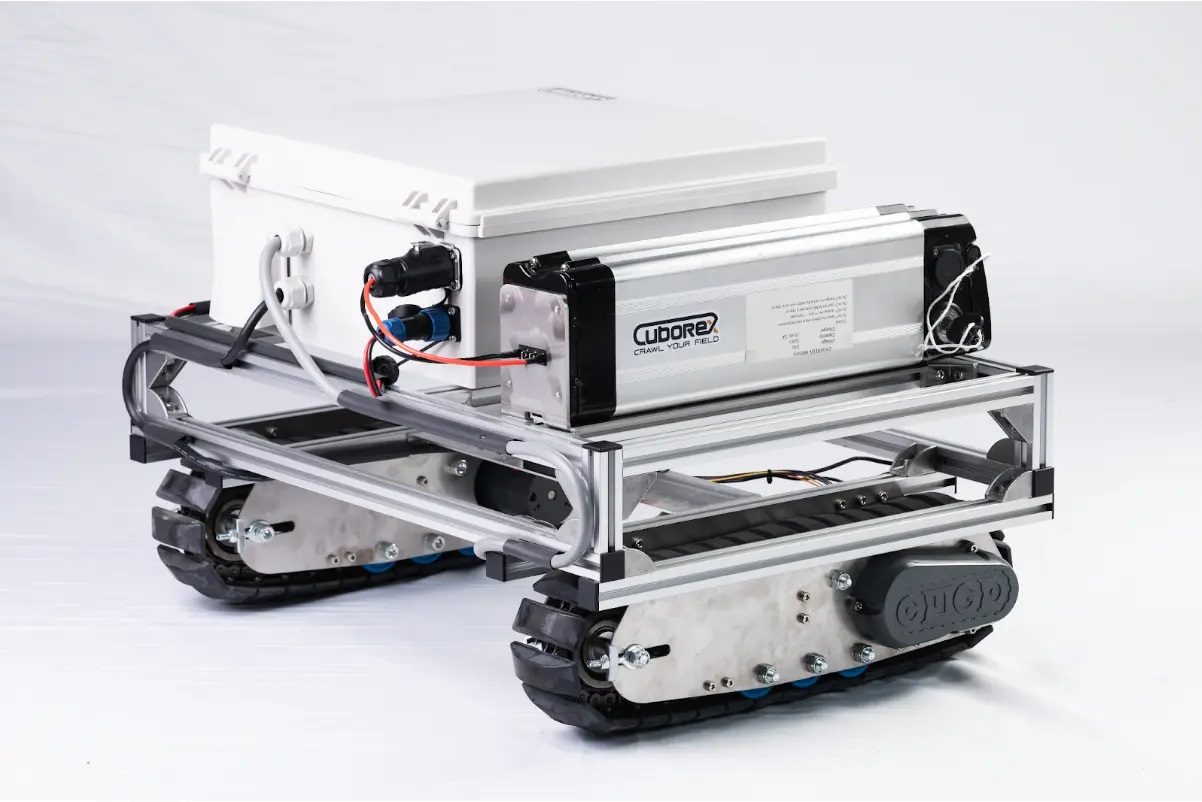
\includegraphics[keepaspectratio,width=70mm]{fig/cugo_ros.jpg}
    \caption{ROS開発キット CuGo V3}
    \label{fig:cugo_ros}
\end{figure}



\subsection{ハードウェア概要}
\begin{figure*}[htbp]
    \centering
    \begin{minipage}[b]{0.45\linewidth}
        \centering
+        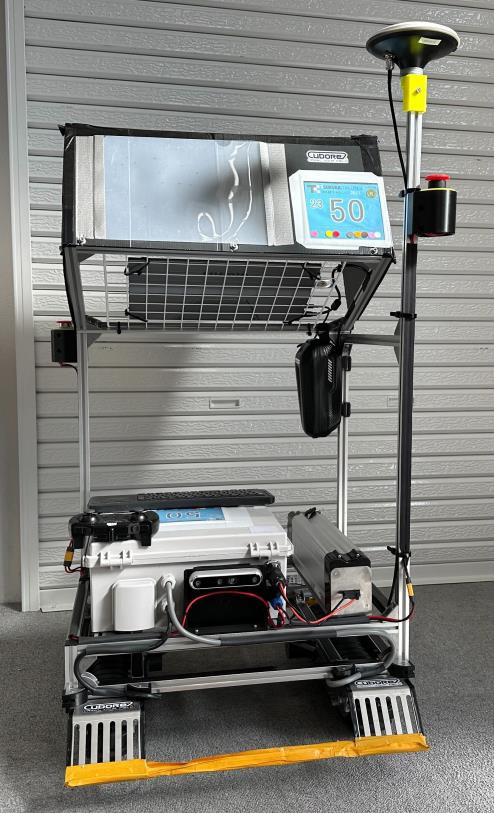
\includegraphics[keepaspectratio,width=70mm]{fig/cugo_tsukuba.png}
        \caption{つくばチャレンジ仕様 CuGo}
        \label{fig:cugo_ros_tsukuba}
    \end{minipage}
    \begin{minipage}[b]{0.45\linewidth}
        \centering
        \caption{ロボット諸元}
        \label{tab:cugo_ros_tsukuba_spec}
        \begin{tabular}{lc}
            \hline
            前長     & 0.7 [m] \\
            全幅     & 0.7 [m] \\
            全高     & 1.3 [m] \\
            重量     & 33  [kg] \\
            最高速度 & 3.5 [m/s] \\
            駆動機構 & クローラ \\
            \hline
        \end{tabular}
    \end{minipage}
\end{figure*}

本年度の実験に使用したロボットの外観を以下の図 \ref{fig:cugo_ros_tsukuba} に示す.ハードウェアの構成を表 \ref{tab:cugo_ros_tsukuba_spec} に示す.つくばチャレンジ走行用ロボットには,CuboRex製自律走行ロボットの開発用プラットフォームである,“ROS開発キット CuGo V3”をベースに課題に必要な装備を追加した.
\subsection{ROS開発キット CuGo V3}
“ROS開発キット”は,汎用クローラユニットであるCuGo V3,それを正確に制御するマイクロコントローラ,ROSを実行するLinuxコンピュータ,それを駆動するバッテリーや電源システムがオールインワンとなったパッケージ製品である.これに必要に応じて3D LiDARやGNSS,カメラなどの装備を加えることで,最小限の労力で屋外を走行するクローラロボットの開発を開始することができる.



\subsection{つくばチャレンジ仕様}
本年度のつくばチャレンジでは,“ROS開発キット”にGNSS,デバッグ用モニター,モニター確認用のひさし,転倒防止用のステー,機体拡張のため押しやすい位置に非常停止スイッチを再設置する変更を行った.後述するが,ナビゲーションシステムに使用したセンサは2DLidar,GNSS,ホイールオドメトリのみという非常にシンプルな構成となっている.計算資源としてもJetson Orin NXというシングルボードコンピュータ1台とモータ制御用のArduino UNO R3のコントローラで構成されており,比較的安価で製造しやすい屋外走行ロボットとなった.

\section{ナビゲーションシステム}
\subsection{ナビゲーション概要}
本年度のつくばチャレンジのナビゲーションシステム構成図を図\ref{fig:system}に示す.このシステムでは,基本的にみちびきのセンチメーター級測位補強信号を使って補正したGNSSの位置を使用して目的地を目指す.
2023年のコースからGNSSの信号を遮る屋根や建物の直下を通るようになったため,対策が必要である.このエリアを通過するとき, 図\ref{fig:cityhall_fix} のようにGNSSの測位精度の悪化を確認できたため,このエリアに限って地図を作成し地図に対して自己位置推定を行った.GNSSを使用しないエリアを通過した後,ふたたびGNSSの自己位置推定に切り替えて走行することにより,大規模な地図を作成することなく長距離の自律走行を実現した.この章では,以下の順番でナビゲーションシステムの詳細について説明する.

GNSSによる自己位置推定
2D MAPによる自己位置推定
センサフュージョン
GNSSとMAPの位置推定の切り替え
Waypointの設定
経路計画
障害物回避
その他開発支援ツール

\begin{figure}[htbp]
    \centering   
    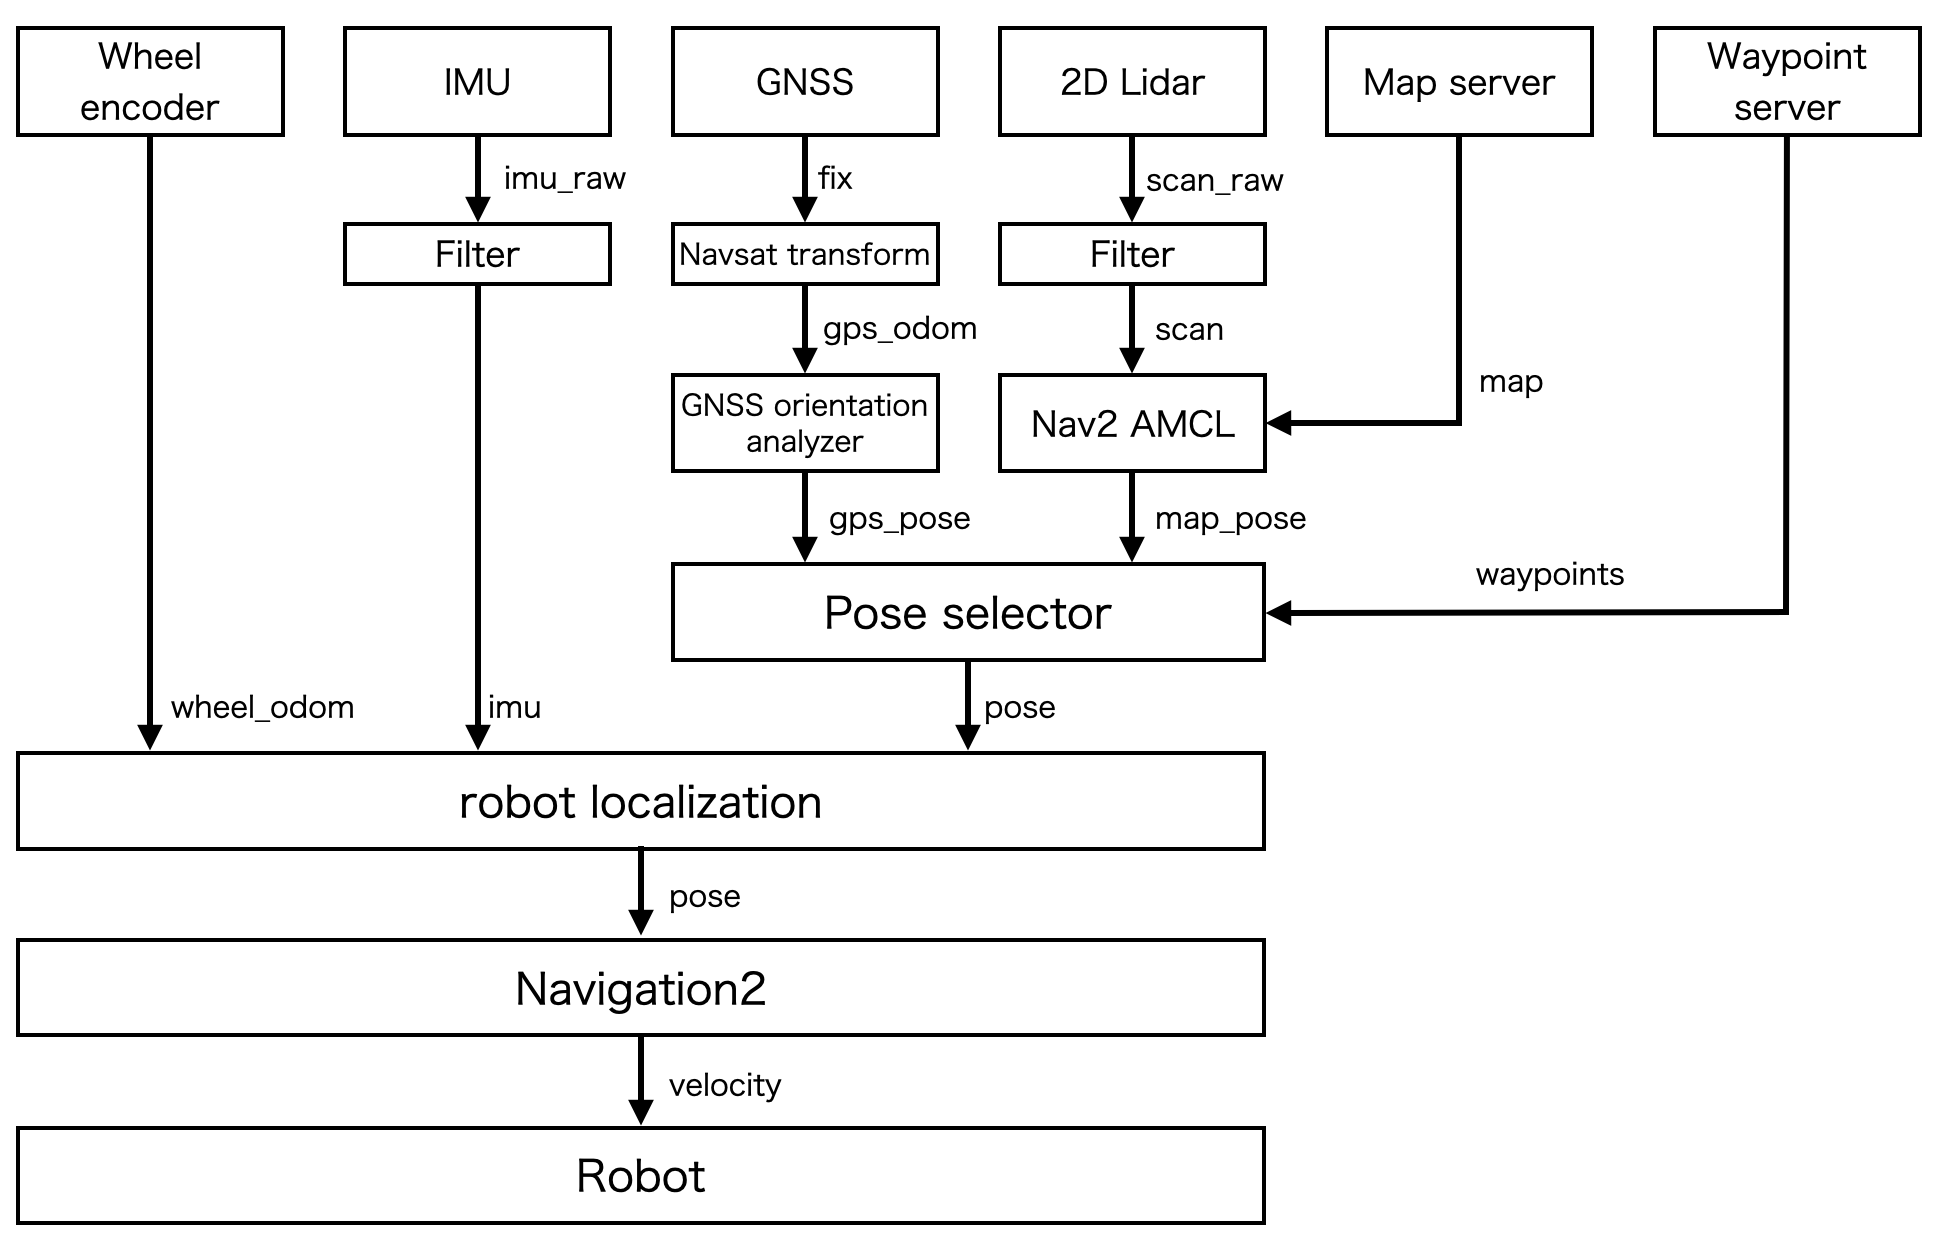
\includegraphics[keepaspectratio,width=80mm]{fig/system.png}
    \caption{ナビゲーションシステム概要図}
    \label{fig:system}
\end{figure}

\begin{figure}[h]
    \centering   
    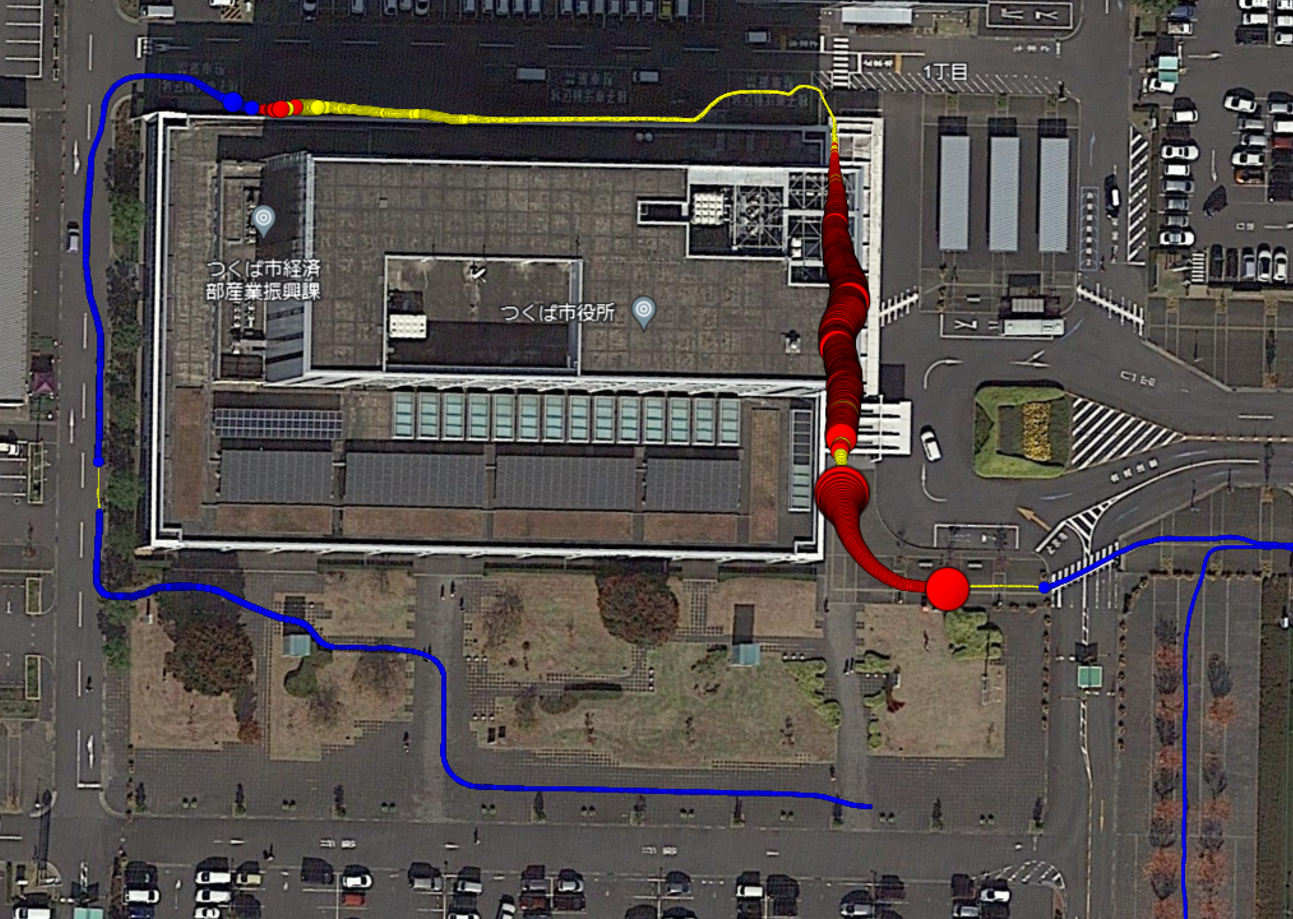
\includegraphics[keepaspectratio,width=80mm]{fig/cityhall_fix.png}
    \caption{確認走行区間のfix状況,青:fix,黄:float,赤:GDPS}
    \label{fig:cityhall_fix}
\end{figure}

\begin{figure}[h]
    \centering   
    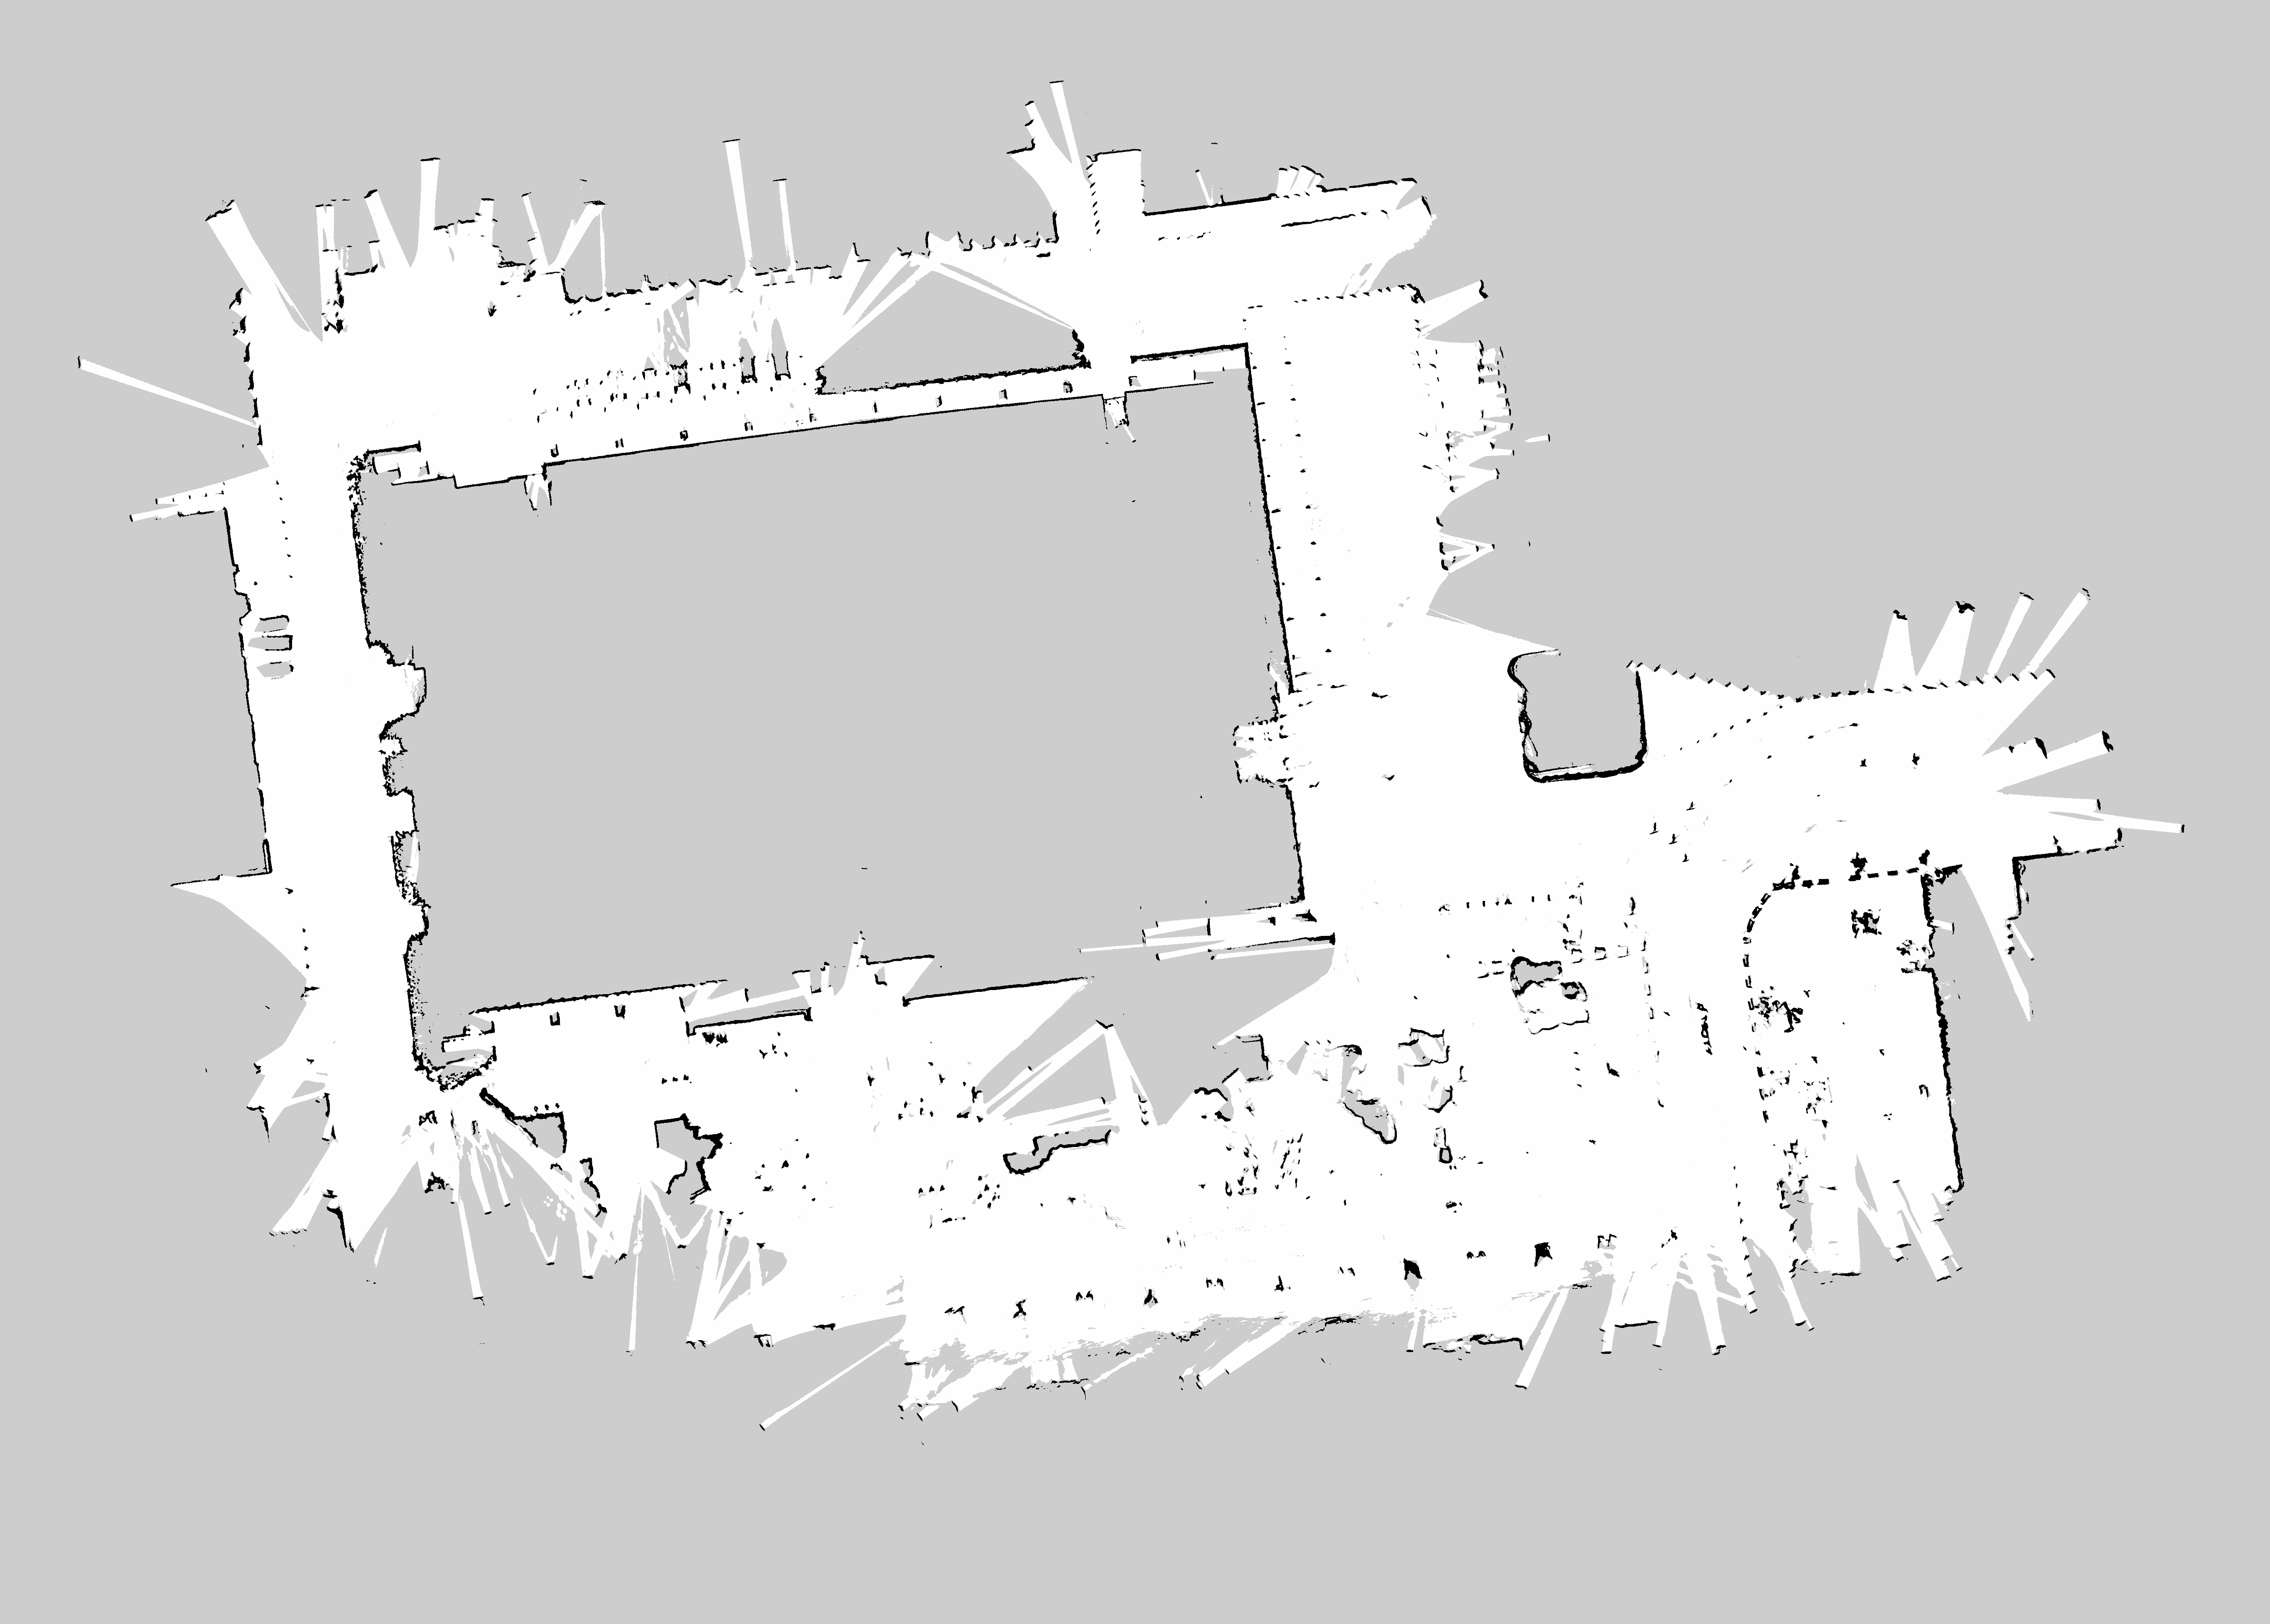
\includegraphics[keepaspectratio,width=80mm]{fig/map.png}
    \caption{作成した確認走行区間の2D地図}
    \label{fig:map}
\end{figure}

\subsection{GNSSによる自己位置推定}
ロボットの内部にCLAS受信モジュールD9CX1とRTKモジュールF9PX1を,機体上部にGNSSアンテナJCA228Eをそれぞれ1組搭載し,CLASによる測位を5Hzで行った.
CLASとはセンチメートル級測位サービスを示し,準天頂衛星みちびきが配信する補強信号を受信することで,日本国内では精度の高い測位が可能となるサービスである.
CLASの移動体における水平方向の測位精度は,$12[\mathrm{cm} (95 \%)]$以下である.
大会においては,本走行コースのゴール地点の緯度・経度 $(36.0826686 ,140.0775115)$ を原点として,測位された緯度・経度との差分を自己位置とした.
ロボットの姿勢角推定は,図\ref{fig:gnss_orientaiton} のように前回時間からの移動量をもとに算出した姿勢を自己位置とした.
ただし,姿勢角の算出は下記の条件を満たす際のみ適用し,それ以外の状況では姿勢角を算出しなかった。
\begin{itemize}
    \item ロボットの直進速度が $0.3[\mathrm{m/s}]$ 以上
    \item ロボットの旋回速度が $0.3[\mathrm{rad/s}]$ 以下
\end{itemize}
姿勢角が算出されない期間における姿勢角の自己位置推定は,後述のセンサフュージョンにより補間した.



\begin{figure}[h]
    \centering   
    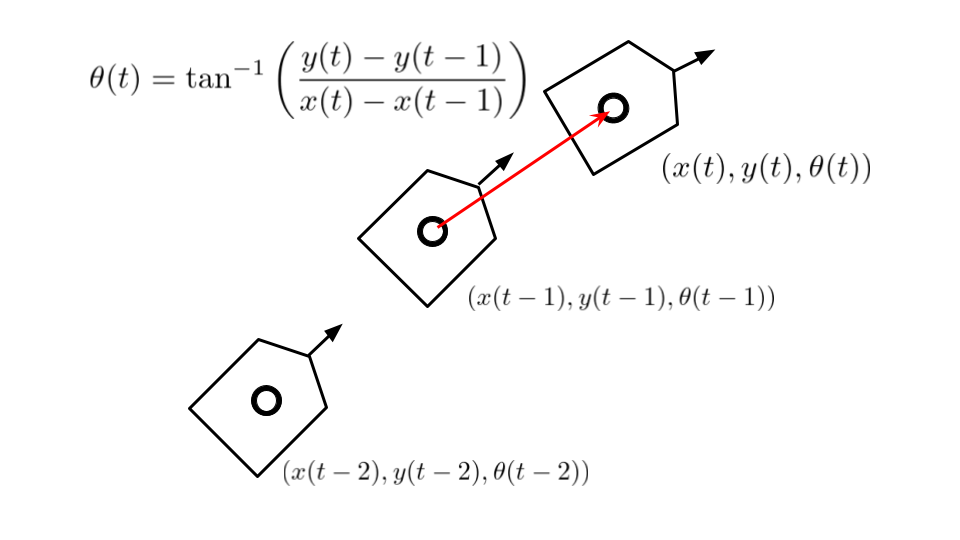
\includegraphics[keepaspectratio,width=80mm]{fig/gnss_orientation.png}
    \caption{GNSSによる姿勢角推定}
    \label{fig:gnss_orientaiton}
\end{figure}

\subsection{2D MAPによる自己位置推定}
ロボット下部に取り付けられた2DLidarを使って図\ref{fig:map}のつくば市庁舎周辺の地図を作成した.2DLidarは地面から120mmの位置に取付てあり,周囲360度,最大30mまでの距離を得ることができる.SLAMはCartographer[9]を利用した.確認走行区間のルートをを1.5周するセンサデータを使い,パラメータを調整して地図を作成した.作成した地図は図Xに示す.実際のナビゲーションでは,北の屋根があるエリアからピロティを抜けた区間まではこの地図の位置を使用した.
(場合によってカットする)地図を作成する際に,ループクローズが発生するが直線の精度が最も高くなるように調整した.この調整をしないと,ループクローズしたときの誤差の勾配がちょうど北エリアで詳細するため,GNSSと地図の位置にずれが発生する.

\subsection{センサフュージョン}
このナビゲーションシステムでは,図\ref{fig:system}のようにロボットの位置推定にホイールオドメトリ,IMU,GNSS,MAP Localizationを入力している.IMUは9軸で地磁気を利用して絶対確を取得していたが,市庁舎北エリアの急速充電器付近で非常に強いノイズを受け屋根ありエリアでの姿勢角の精度悪化が無視できないため共分散を無限大に設定していて,実質使用していない.

ホイールオドメトリの値は,作動二輪モデルから nav msgs Odometryの値を算出して利用している.GNSSの姿勢は前項の通り,直前の連続した位置からロボットの向いている方向を推定しnav msgs Odometryに格納している.MAP Localizationはnav2 AMCLを利用している.AMCLの自己位置推定結果はtfでの出力は無効化して,nav msgs Odometryに変換して利用している.

3つの nav msgs Odometry をrobot localization[10]パッケージを利用してEKF処理をし,ロボットの自己位置としてナビゲーションに利用している.

\subsection{GNSSとMAPの位置推定の切り替え}
ナビゲーション構成図のPose Selectorが示す部分で上記3.2と3.3の各自己位置推定をした値を排他的に選択し,EKFに送る.こうすることで,センサフュージョンをする側のノードでは,現在の状態がGNSSであるかMAPであるかを意識することなく機械的に処理することができる.それぞれの状態は次に向かうWaypointのデータ構造にフラグとして内包しており,Waypointごとにどちらの位置を使用するかを記録することで切り替えを実現している.

\subsection{Waypontの設定}
Waypointの設定はロボットの自己位置をそのまま記憶するツールを作成した.GNSSとMAP Localizationのどちらの状態であっても,先述の通り,ロボットが認識する自己位置は変わらないため,現在認識している自己位置をそのままキーボード操作をトリガーにcsvファイルに記憶する.実験走行では,当日の午前にロボットをコントローラでマニュアル操作し,走行させたい経路の2mおきのWaypointを記憶させた.午後に検定を実施し,作成したWaypoint列のcsvファイルをナビゲーションシステムに読み込ませて自律走行を行った.

\subsection{経路計画}
ロボットの自己位置からWaypointまでの走行経路の生成は,ROS 2標準のNavigation2[11]をそのまま利用した.Waypointまでの経路はA*アルゴリズム[12]で算出し,その経路をRegulatedPurePersuit[13]で追従した.

\subsection{障害物回避}
障害物の回避には2DLidarを使用し,ROS 2標準のNavigation2[11]によるものをそのまま利用した.
しかし,2DLiDRを使用しているためパイロンのような起伏のある形状の障害物を回避できない,経路生成が行われるより前に衝突する箇所に障害物が発生した際に避けられない,という問題があった.
そのため,前述の機能に加えて,経路生成より高速で処理が可能な障害物判定機能を追加した.
具体的な処理は,コストマップで機体前方の5点を常に参照し,定点のコストが閾値以上となった際には停止させるものとした.
この閾値を低くすることで障害物に対する接近を抑制することが可能となり,起伏のある形状の障害物にも接近せず,衝突を回避できた.

\subsection{その他開発支援ツール}
現場でのロボットのデバッグは,さまざまな条件の中で何が起きたかを素早く発見し,迅速に修正することが大切である.

ロボットの状態確認としては、1  次の目標のWaypointのID 2  フラグ管理で正常でない組み合わせが発生したことの通知 3)センサや中間ノードからトピックが来なくなった時の通知,を読み上げツールによってロボットにしゃべらせた.これにより,異常なゴール判定,想定できなかった状態遷移,各種機能の失陥をいち早く知ることができ,対策を本走行当日までに適用することができた.読み上げツールはOpenJTalk[12]を使用し,文字列のトピックを受け取るとそのまま読み上げるアプリケーションを作成し,ロボットに搭載されたディスプレイのスピーカーから音声を再生することで実現した.

\section{性能評価}
\subsection{ハードウェア走行性能}
走行ハードウェアとしては,CuboRex製のクローラユニットであるCuGo V3を使用した.研究学園前公園の階段の乗降はできないが,必須課題の走行コースで問題になる段差はなかった.7 15の実験走行では,炎天下の中必須課題の走行コースをマニュアル走行で4周したが,ハードウェアでのトラブルはなかった.

\subsection{GNSS位置推定}
今回の手法を使用することで,市庁舎北とピロティの区間以外のコース区間では指定した通りの自律走行が実現できた.
上記区間を除けば,本走行,試走会ともに自己位置のロストを起因とする走行失敗・大きなルート逸脱は発生しなかった.
しかし,同じ経路を指定して自律走行をさせた際に,最大 $1[\mathrm{m}]$ 程走行経路のずれが発生した.
これは上位システムに起因する要素と,天気や湿度,準天頂衛星を含む測位衛星の位置といった,環境の変化が原因だと考えられる.
つくばチャレンジの課題達成においては問題ない範囲の誤差であったが,狭路を含むルートの走行をこなすためには,3D Mappingのような他の手法を併用する必要がある.

一方,市庁舎北とピロティの区間においては指示通りの自律走行は難しく,必ず市庁舎の壁から離れる方向に進んでしまった.
これは,市庁舎のない方向からのマルチパスにより,自己位置が実際よりも市庁舎側に寄った位置にいると誤認してしまったためと考えられる.
前述の通り,電波を遮蔽する物体が存在する環境においては本手法による自己位置推定は難しいため,ロボットの使用環境の調査と,遮蔽物が存在する場合は代替手法の検討が必須である.

\subsection{2D MAP位置推定}
図Xに示すつくば市庁舎北エリアの区間はAMCLによる自己位置推定を使用している.図Xで示した作成した地図では,1) 図Xの位置に商用バンが止まっていた時に著しく位置精度が低下した 2) 図Xの位置で1度だけ点対象の位置に誤マッチングした,ことがあった.いずれも確率は低かったが,あらゆるシーンで走行可能にするには,3Dにすることやもっと遠くの地形を見ることなどの工夫が必要であると感じた.

\subsection{障害物回避}
屋内・屋外のコンクリート床の上で下記試験が達成できるように,コストを参照する点の位置,障害物の有無を判定する閾値の調整した.
\begin{itemize}
    \item 走行可能部が機体幅とほぼ同等となる $1.2[\mathrm{m}]$の幅にパイロンを設置し,その間を自律走行で通過できる
    \item 機体が直進走行中に機体の前方  $0.5[\mathrm{m}]$の位置にパイロンを設置し,衝突することなく停止できる
\end{itemize}

\section{本走行の結果}
本走行では,確認走行区間を超えた先のパイロン地帯でパイロンを避けずに停止してしまったため走行を断念した.パイロンを避けきれなかった原因としては,以下の原因が考えられる.

経路計画の動作周波数が1Hzであり,パイロンを回避する経路が引かれる前にロボットが走行を続けた.もとより,GNSSのみでどこまで走行できるかを主眼として開発を進めていた時期があり,GNSSとMAP Localizationが同居することを想定していなかった.本番直前にシステムを大幅に肥大化させたことにより,最適化が進まず計算資源不足に陥ってしまったため,さまざまな制御周期を下げる対応をした.これにより,経路計画の動作周波数が1Hzとなってしまい,回避行動をとる前に障害物を認識する前の行動を続けてしまった.また,周囲の障害物を避けるコストマップの範囲も大幅に小さく設定したため,ロボットが障害物を発見するのにより障害物に近づいた状態でないと障害物に気づけない状況になっていた.

ロボットが他のロボットなどの障害物を回避する手段として,積極的に回避することをせずにその場でとどまることを選択してしまった.回避行動をとっていればとどまることはないが,回避行動をとることができず,この仕様によってデッドロックしてしまった.

Waypointを疎に打ちすぎていた.確認走行区間では,周囲のロボット以外の障害物は明確に知ることができており,Waypointを1.5mおきに密に設置し走行経路を明確に定義することで安定した走行を実現していた.しかし,パイロン区間は日によってパイロンの設置位置が変わるため,Waypointの密度を10m以上の疎な設定していた.これによりパイロンから積極的に離れる経路にはならず,繰り返しパイロンに向かって走行する挙動をしてしまった.

当日のGNSSの値が最大0.5mほどずれていた.GNSSの値は以前より比較的高精度に位置推定をすることができるようになったが,衛星の位置によっては誤差が大きい時間帯が存在する.ロボットが停止してしまった区間は理想的なオープンスカイな環境ではあったが,もとから設定したWaypointの位置より0.5m程度北にずれた位置を走行していた.パイロン地帯でも比較的設置されにくい点字ブロックに沿って走行をする経路を設定したが,そこから北にずれた経路を走行していたため積極的にパイロンが多い経路を走行し,パイロンを避けきれないケースが発生した.

パイロンを避けられなかった直接的な原因は以上の4点が挙げられるが,確認走行区間の先の対応をしたのが実験走行の最終日の午後のみで試行回数が圧倒的に少なかった.この先のほとんどの区間がオープンスカイな理想的な環境であり,運用次第では2DLidar+GNSS+ホイールオドメトリのみという非常にシンプルな構成でもっと距離を伸ばせたと考える.この先の区間でしか現れない問題を収集できなかった点が今回の課題である.

\section{結言}
本年度のつくばチャレンジの取り組みとして,つくばの市街地で走行できるロボットハードウェアを作成し,GNSSとMAP Localizationの位置推定を任意のタイミングで切り替えることができるナビゲーションシステムを作成し検討した.

走行実験では,確認走行区間の走行を実験走行最終日の検定と本走行を連続で達成した.しかし,その先の走行区間の調整や設定まで至れなかったため,パイロン区間で停止した.シンプルな構成で自律走行するシステムを実現したが,計算能力の限界や動的物体の障害物回避などに課題が残る.そのため,多くの現場で走行できるシステムにするためには最適化や計算資源の見直し,より広い範囲を認識することができるセンサ追加など,必要に応じて資源を増設できるシステムになるように開発を続けたい.

文献



% \section{はじめに}
% \pkg{RBProceedings}文書クラスはW3Cにより策定されている『日本語組版の要件』\cite{JLREQ}に準拠することを目指す\pkg{jlreq}クラスをベースにしている.
% ただし,本文書クラスでは紙面スペースの都合上,多くの余白値をかなり詰めるように設定しており,例えば行間は\ruby{外国人参政権}{がい|こく|じん|さん|せい|けん}のようにルビを振れる最小限の余白に設定してある.

% 論文では,単純なテキストのみならず,しばしば数式
% \begin{equation}
% P(B\mid A) = \frac{P(A\mid B)P(B)}{P(A)}
% \end{equation}
% や箇条書き
% \begin{itemize}
% \item 第1の項目
% \item 第2の項目
% \end{itemize}
% といった構造も用いられるが,これらもよく知られた文書クラス(例えば\pkg{jsarticle}等)と同様のシンタックスで利用できる.

% \section{図表の挿入}
% 図表についても通常の \LaTeX と同じ方法を用いることができる.

% \subsection{図について}
% 図の挿入は,通常\pkg{graphicx}パッケージによって行う(図\ref{fig:sample}).
% クラスオプションにワークフロー(\code{dvipdfmx}等)を指定していれば,
% 各パッケージを読み込む際に何度も同じオプションを指定する必要はない.

% \begin{figure}[t]
% \centering
% \includegraphics[width=6cm]{example-image-a}
% \caption{図の例}
% \label{fig:sample}
% \end{figure}

% \subsection{表について}
% 表の挿入は,\verb|\begin{table}...\end{table}|環境を使う(表\ref{tab:sample}).

% \begin{table}[t]
% \centering
% \caption{表の例}
% \label{tab:sample}
% \begin{tabular}{llcc}
% \hline
% 日本語 & Japanese & ほげほげ & ふげふげ \\
% 英語 & English & hogehoge & fugefuge \\
% \hline
% \end{tabular}
% \end{table}

% \section{参考文献}
% 参考文献の参照例.
% \begin{itemize}
% \item 論文誌の参照例 \cite{Article_01}
% \item 本の参照例 \cite{Book_02}
% \item 国際会議の参照例 \cite{Inproc_03}
% \item 技術報告の参照例 \cite{Techrep_05}
% \item Webページの参照例 \cite{Web_06}
% \end{itemize}

% \section{Writing in English}
% This paragraph shows an English sample.
% There is no problem with writing your manuscript in English.
% If you write in LaTeX, please use the distributed document class with the \code{english} option:
% \begin{quote}
% \verb|\documentclass[|\\
% \verb|  platex,dvipdfmx,english]{rbproceedings}|
% \end{quote}

% % 参考文献
% \bibliographystyle{junsrt}
% \bibliography{myrefs}

\end{document}
